algorithm:
\begin{enumerate}
	\item Calculate $ \hat{\vec{E}}_{0, \bot}^{ijn} $ via discrete Fourier transforms in time.
	\item Calculate $ \bar{\vec{E}}_{0, \bot}^{ijn} $ via two-dimensional discrete Fourier transforms in transverse space.
	\item Calculate transverse electric field components at the boundary.
	\item Calculate longitudinal electric field components the boundary.
	\item Calculate the magnetic field at the boundary.
	\item Calculate $ \hat{\vec{E}}_{\mathrm{B}}^{ijn} $, $ \hat{\vec{B}}_{\mathrm{B}}^{ijn} $ via two-dimensional inverse discrete Fourier transforms.
	\item Calculate $ \vec{E}_{\mathrm{B}}^{ij}(t) $, $ \vec{B}_{\mathrm{B}}^{ij}(t) $ for any given time $ t \in [t^{1} - \frac{z_{\mathrm{B}} - z_{0}}{c}, t^{N_{t}}  - \frac{z_{\mathrm{B}} - z_{0}}{c}] $.
\end{enumerate}

\noindent
implementation:
\begin{itemize}
	\item 2D version of algorithm, Ey, Bx, Bz omitted (identically equal to 0) 
	\item Code written in C++, object oriented to be easily extended to 3D, compiled to static library
	\item Linked into EPOCH as a static library (in order not to disturb the code, for this reason also added support for CMake – machine independent)
	\item Parallelized using hybrid techniques (OpenMP + MPI – computation time in most cases negligible in comparison with the main simulation)
	\item Fourier transforms can be computed using Intel MKL library, FFTW library or without any library (compile time option)
	\item Computed fields dumped into shared files using binary coding (speed up output, save disk storage)
	\item Only transverse component of electric field (Ex) passed to the EPOCH at each time step (no significant slowdown or memory overhead), other fields computed by EPOCH
	\item All new parameters needed for tight-focusing (w0, focal length, etc.) may be specified via input file
	\item Implementation works generally regardless the number of lasers in the simulation or boundaries that they are attached to
\end{itemize}

\noindent
parameters:
\begin{enumerate}
	\item laser:
	\begin{itemize}
		\item wavelength: 1.0 micron
		\item amplitude: 1e15 V/m
		\item duration: 20 fs (in FWHM)
		\item beam waist in focus: 0.7 micron
		\item focus distance from boundary: 8 micron
		\item polarization: p
		\item boundary: x min 
	\end{itemize}
	\item domain:
	\begin{itemize}
		\item x min: -8 micron
		\item x max: 8 micron
		\item y min: -8 micron
		\item y max: 8 micron
		\item nx: 1600 cells (dx = wavelength/100)
		\item ny: 1600 cells (dy = wavelength/100)
		\item dt: 1/(sqrt(2)*c)*wavelength/100
		\item simulation time: 150 fs
	\end{itemize}
\end{enumerate}

To demonstrate drawbacks of the paraxial approximation as well as to evaluate the correctness of the algorithm presented in the previous section of this chapter, several test simulations have been performed. In the following text, a two limit cases are presented. The first simulation employs tightly focused Gaussian laser beam, with the size of the focus comparable with the center laser wavelength, whilst the second one shows the case of the Gaussian beam with the size of the focus one order of magnitude larger than the center laser wavelength, where both approaches should return identical results.

 

\floatsetup[figure]{style=plain, subcapbesideposition=top}
\begin{figure}[h!]
	\centering
	\sidesubfloat[]{{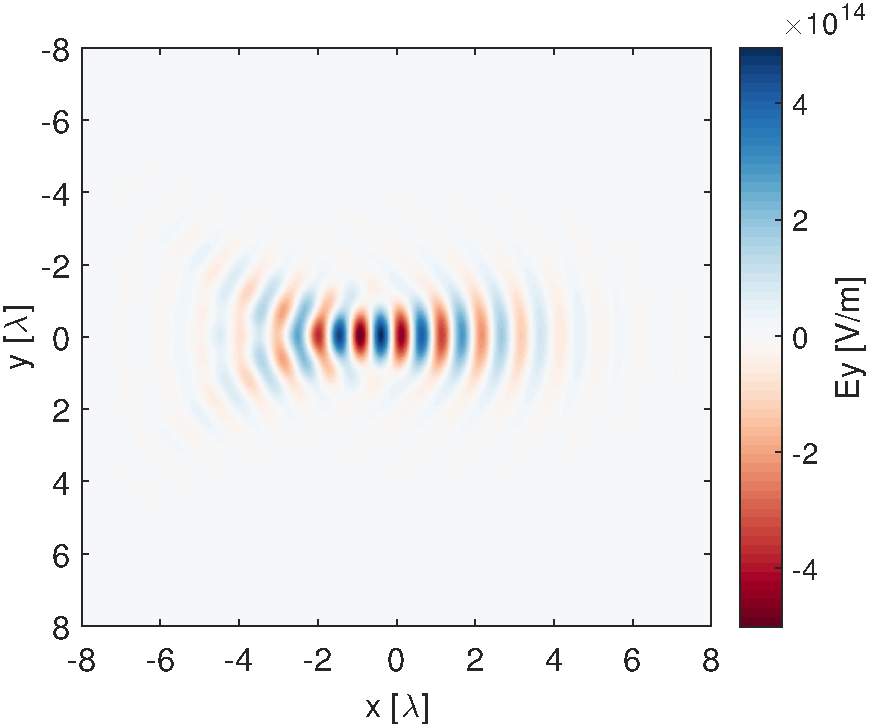
\includegraphics[width=0.44\linewidth]{./img/parax/Ey_focus.pdf}}}
	\hspace{2mm}
	\sidesubfloat[]{{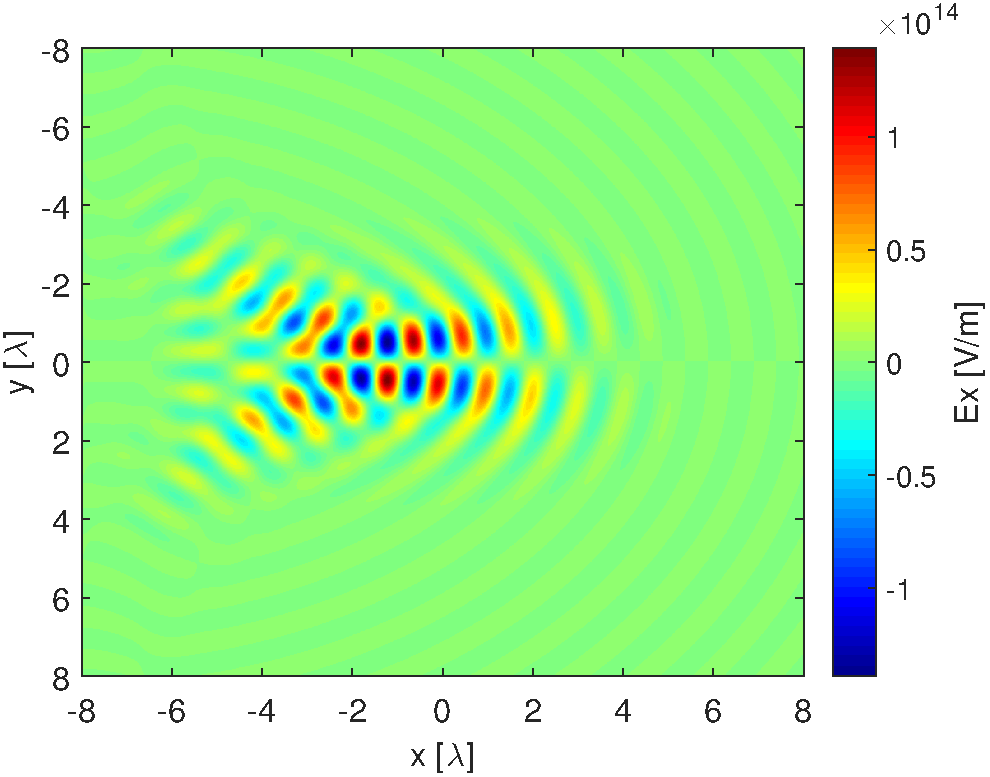
\includegraphics[width=0.44\linewidth]{./img/parax/Ex_focus.pdf}}}\\
	\sidesubfloat[]{{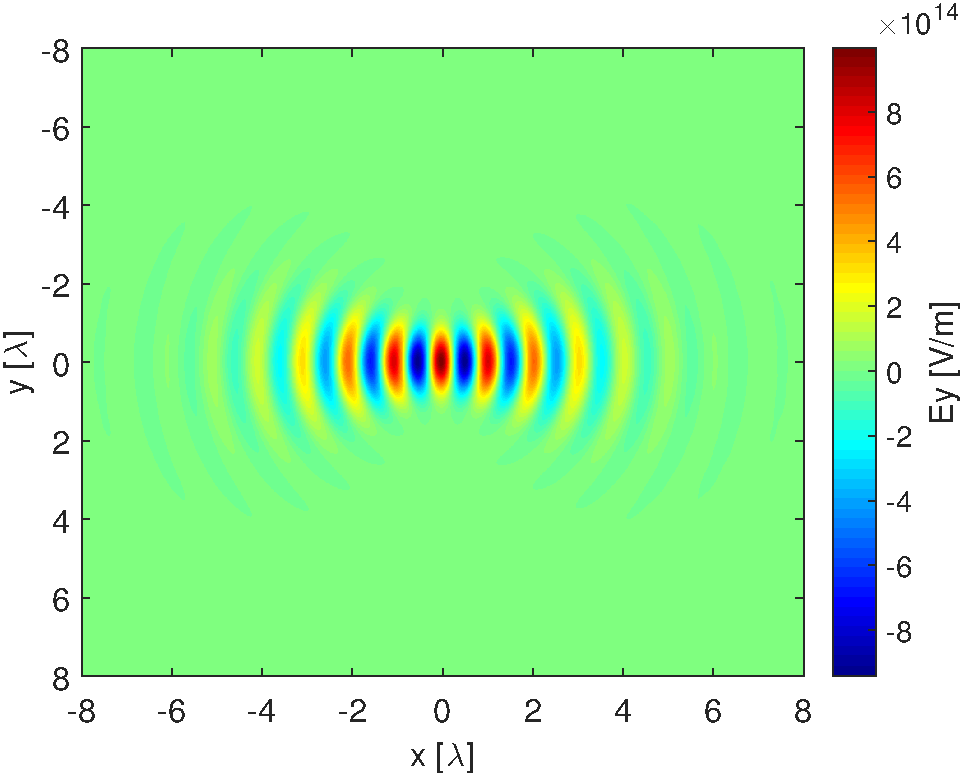
\includegraphics[width=0.44\linewidth]{./img/lbcs/Ey_focus.pdf}}}
	\hspace{2mm}
	\sidesubfloat[]{{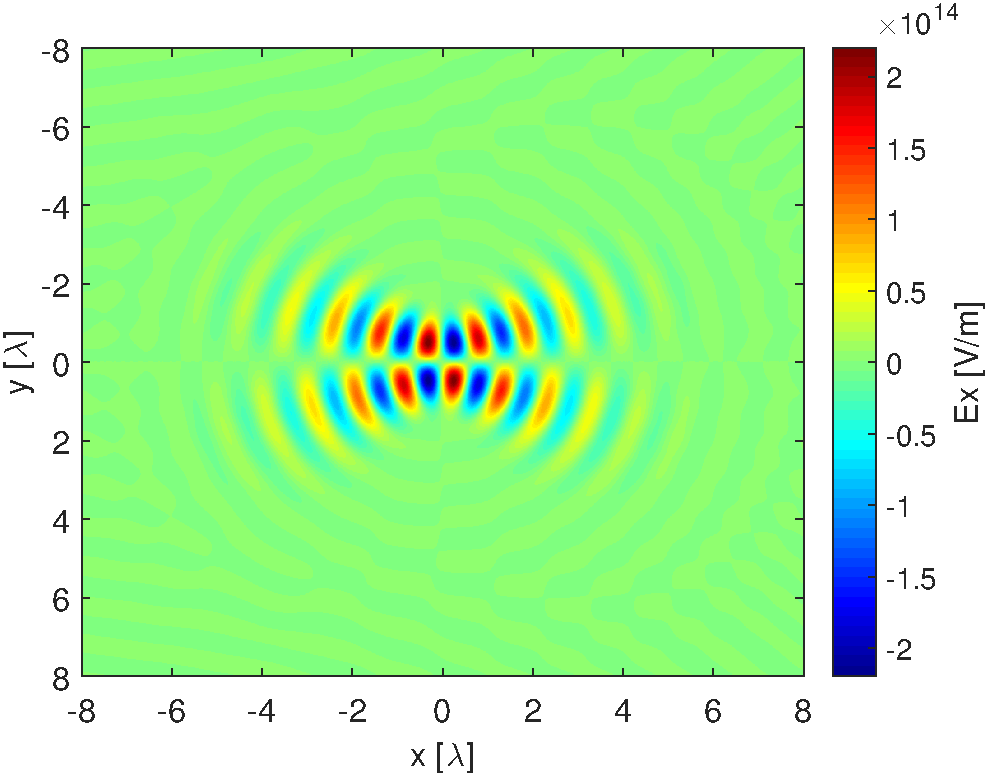
\includegraphics[width=0.44\linewidth]{./img/lbcs/Ex_focus.pdf}}}
	\caption{Transverse ($ E_{y} $) and longitudinal ($ E_{x} $) electric laser field components captured at the time step of their maximal intensity in the focal spot. The cases \textbf{(a)}, \textbf{(b)} correspond to the laser pulse propagating under the paraxial approximation, whilst \textbf{(c)}, \textbf{(d)} come from the simulation where the beam propagation has been resolved within the Maxwell consistent approach. In the case of paraxial approximation, both components reveal strong distortions and asymmetry, their focal spot is located about $ \mathrm{1 \mu m} $ closer to the left boundary than specified and the corresponding amplitude is significantly higher. The laser has been attached to the left hand side boundary.}
	\label{fig:1}
\end{figure}

\floatsetup[figure]{style=plain, subcapbesideposition=top}
\begin{figure}[h!]
	\centering
	\sidesubfloat[]{{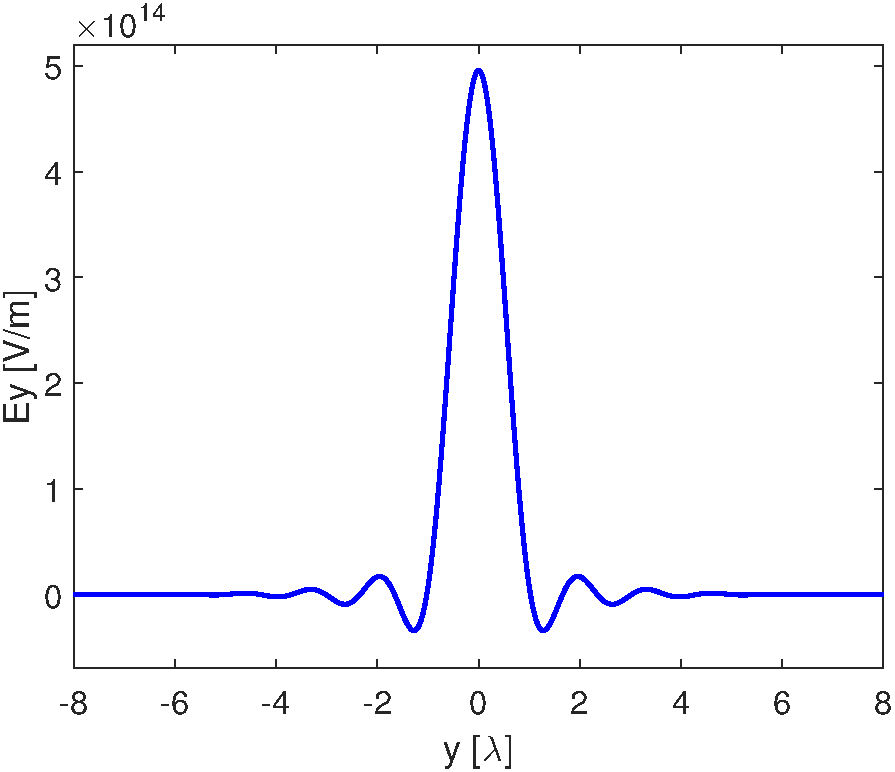
\includegraphics[width=0.4\linewidth]{./img/parax/Ey_focus_trans.pdf}}}
	\hspace{5mm}
	\sidesubfloat[]{{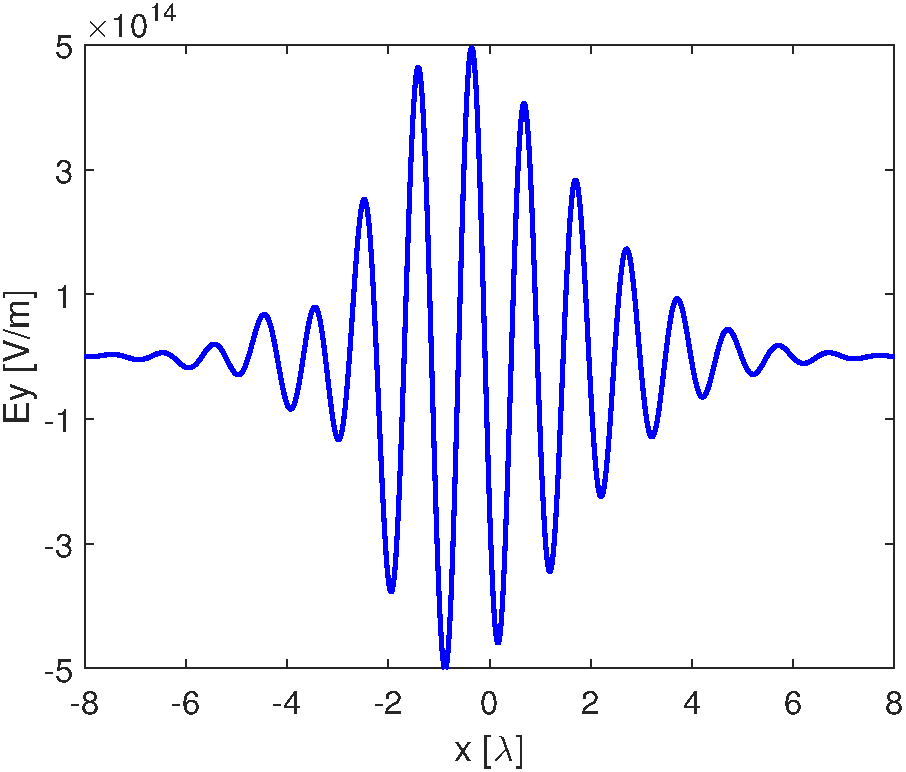
\includegraphics[width=0.4\linewidth]{./img/parax/Ey_focus_long.pdf}}}\\
	\sidesubfloat[]{{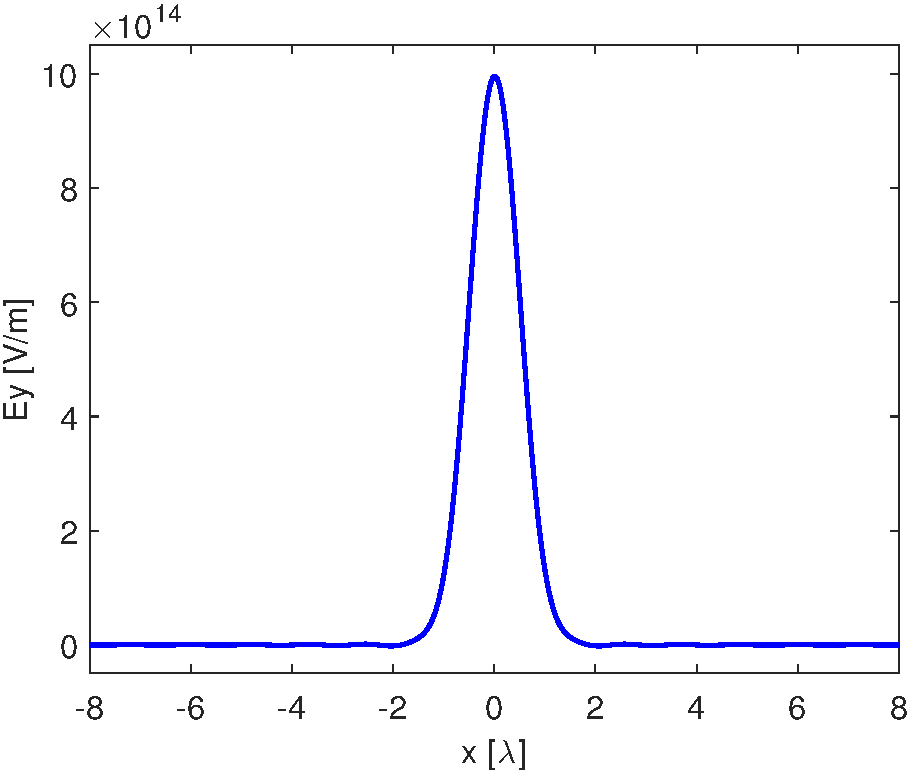
\includegraphics[width=0.4\linewidth]{./img/lbcs/Ey_focus_trans.pdf}}}
	\hspace{5mm}
	\sidesubfloat[]{{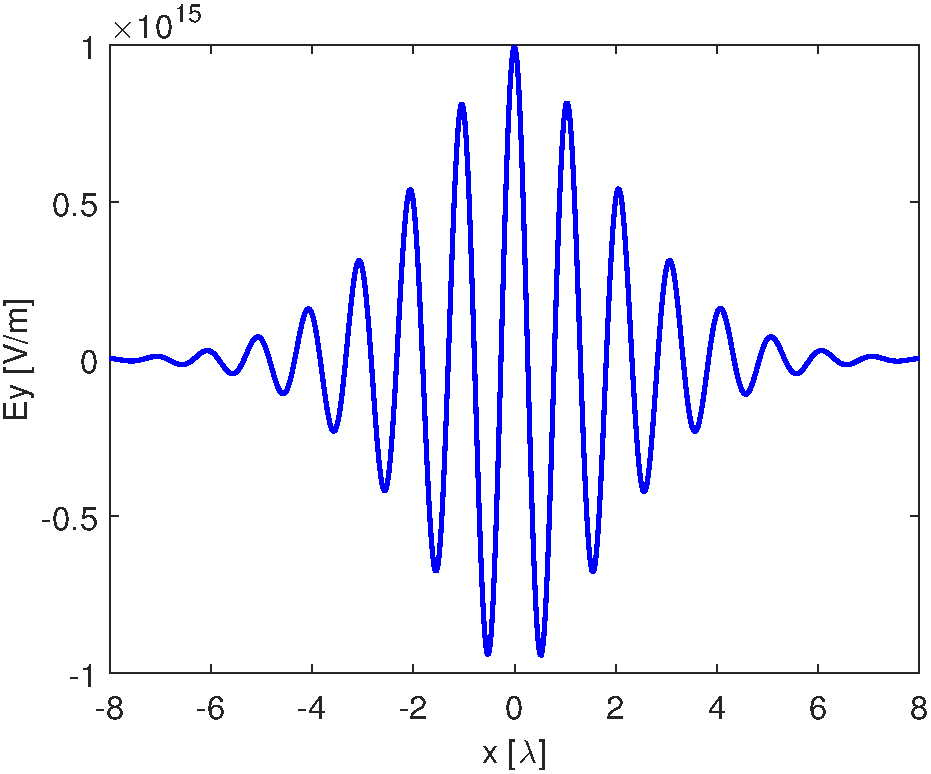
\includegraphics[width=0.4\linewidth]{./img/lbcs/Ey_focus_long.pdf}}}
	\caption{Transverse \textbf{(a)}, \textbf{(c)} and longitudinal \textbf{(b)}, \textbf{(d)} slices of the transverse electric laser field ($ E_{y} $) at the time step when it reaches maximal intensity in the focal spot. The cases \textbf{(a)}, \textbf{(b)} correspond to the laser pulse propagating under the paraxial approximation, whilst \textbf{(c)}, \textbf{(d)} come from the simulation where the beam propagation has been resolved within the Maxwell consistent approach. In the case of paraxial approximation, one can clearly see strong side-wings in the spatial beam profile \textbf{(a)} as well as the asymmetry of the field in the longitudinal line-out \textbf{(b)}.}
	\label{fig:2}
\end{figure}

\floatsetup[figure]{style=plain, subcapbesideposition=top}
\begin{figure}[h!]
	\centering
	\sidesubfloat[]{{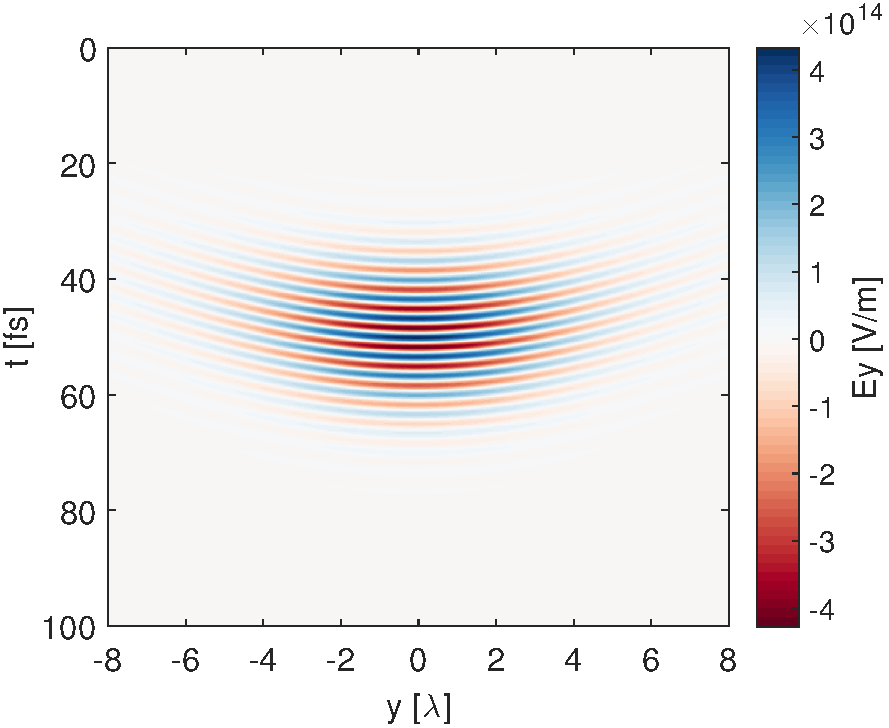
\includegraphics[width=0.44\linewidth]{./img/lbcs/Ey_boundary_time.pdf}}}
	\hspace{2mm}
	\sidesubfloat[]{{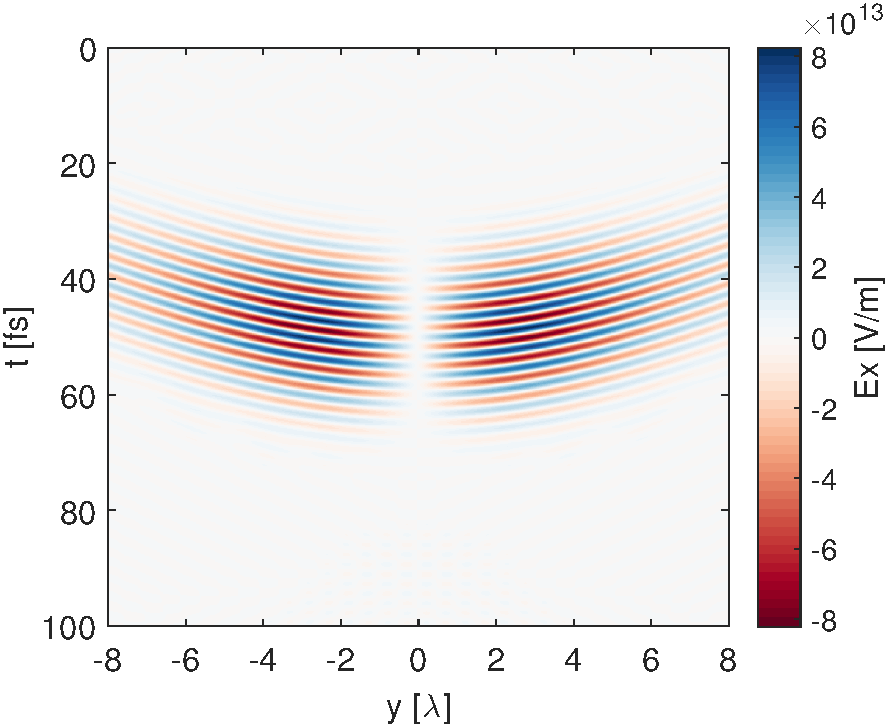
\includegraphics[width=0.44\linewidth]{./img/lbcs/Ex_boundary_time.pdf}}}
	\caption{The time evolution of transverse ($ E_{y} $) \textbf{(a)} and longitudinal ($ E_{x} $) \textbf{(b)} electric laser field components at the boundary that the laser is attached to. Both components has been calculated according to the Maxwell consistent approach.}
	\label{fig:3}
\end{figure}

\floatsetup[figure]{style=plain, subcapbesideposition=top}
\begin{figure}[h!]
	\centering
	\sidesubfloat[]{{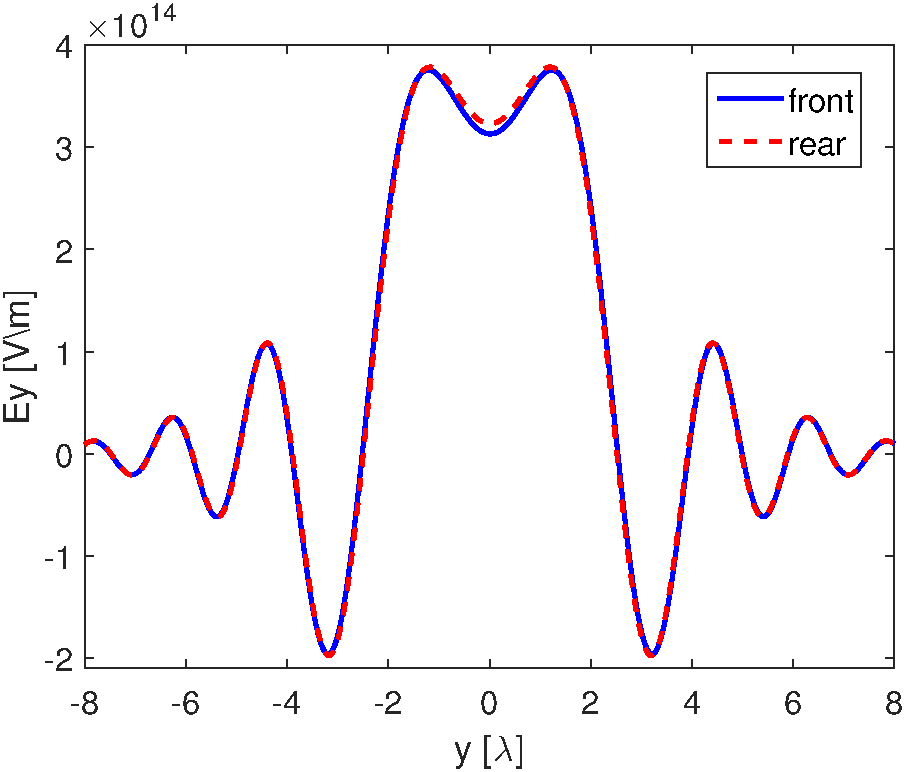
\includegraphics[width=0.4\linewidth]{./img/lbcs/Ey_boundary_trans.pdf}}}
	\hspace{5mm}
	\sidesubfloat[]{{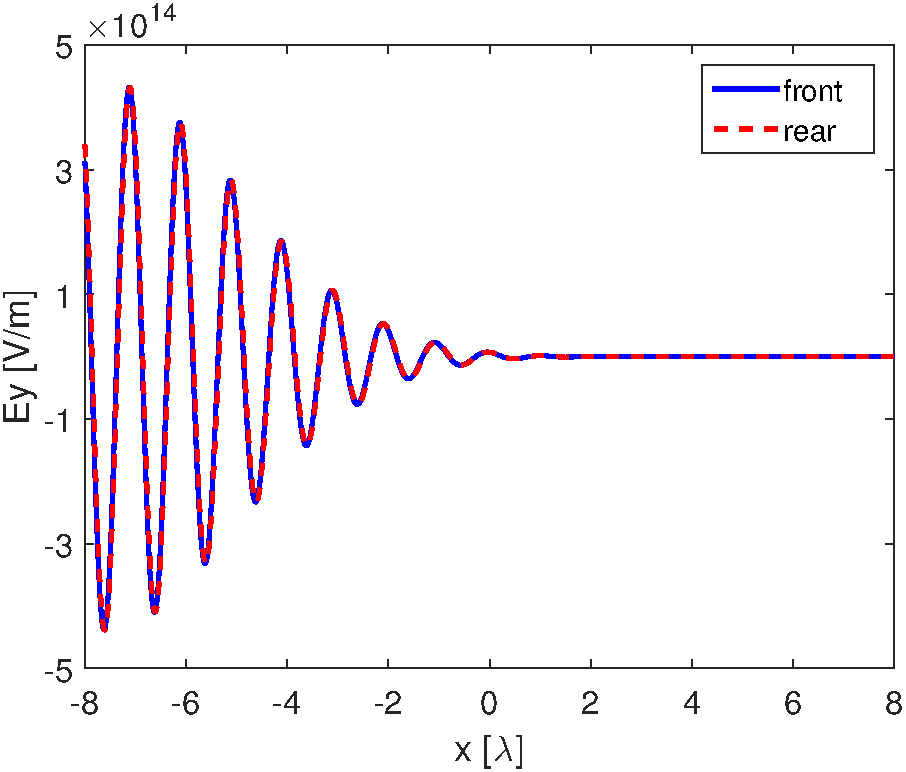
\includegraphics[width=0.4\linewidth]{./img/lbcs/Ey_boundary_long.pdf}}}
	\caption{Transverse \textbf{(a)} and longitudinal \textbf{(b)} slice of the transverse electric laser field ($ E_{y} $) when it reaches its maximal intensity at the front (blue) and rear (red) boundary. The results come from the simulation where the Maxwell consistent approach for laser propagation has been used. For better comparison, the field at the rear boundary in \textbf{(b)} has been horizontally flipped. The exact match between the field shapes at a different time steps of simulation proves the correctness of the laser beam propagation.}
	\label{fig:4}
\end{figure}

\floatsetup[figure]{style=plain, subcapbesideposition=top}
\begin{figure}[h!]
	\centering
	\sidesubfloat[]{{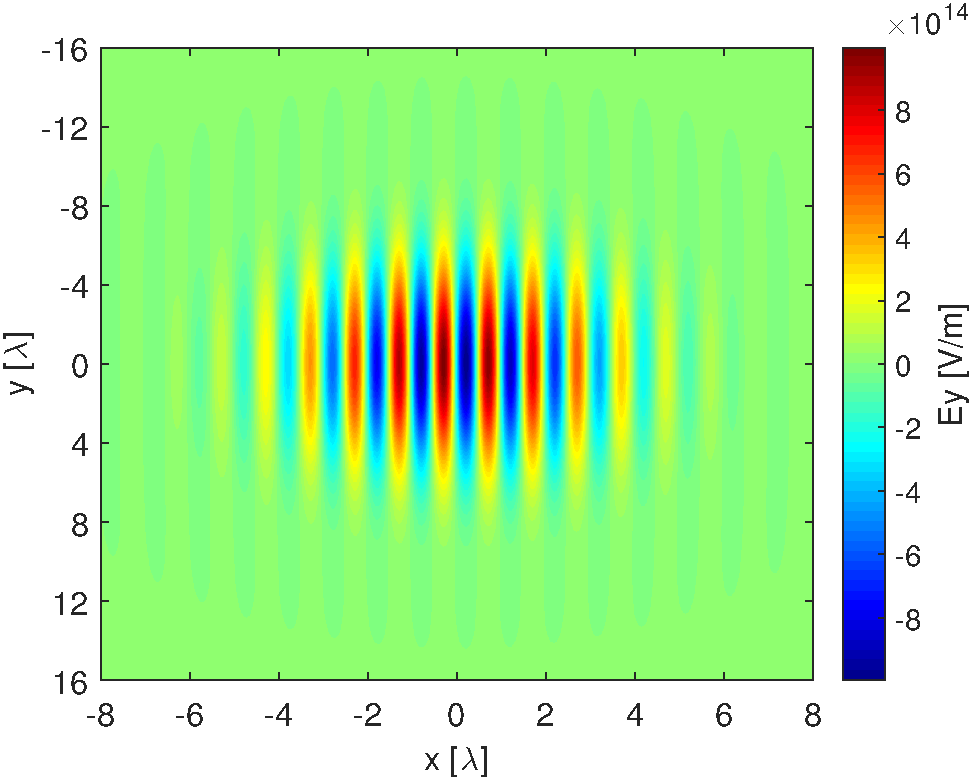
\includegraphics[width=0.45\linewidth]{./img/parax/Ey_focus_5mic.pdf}}}
	\hspace{2mm}
	\sidesubfloat[]{{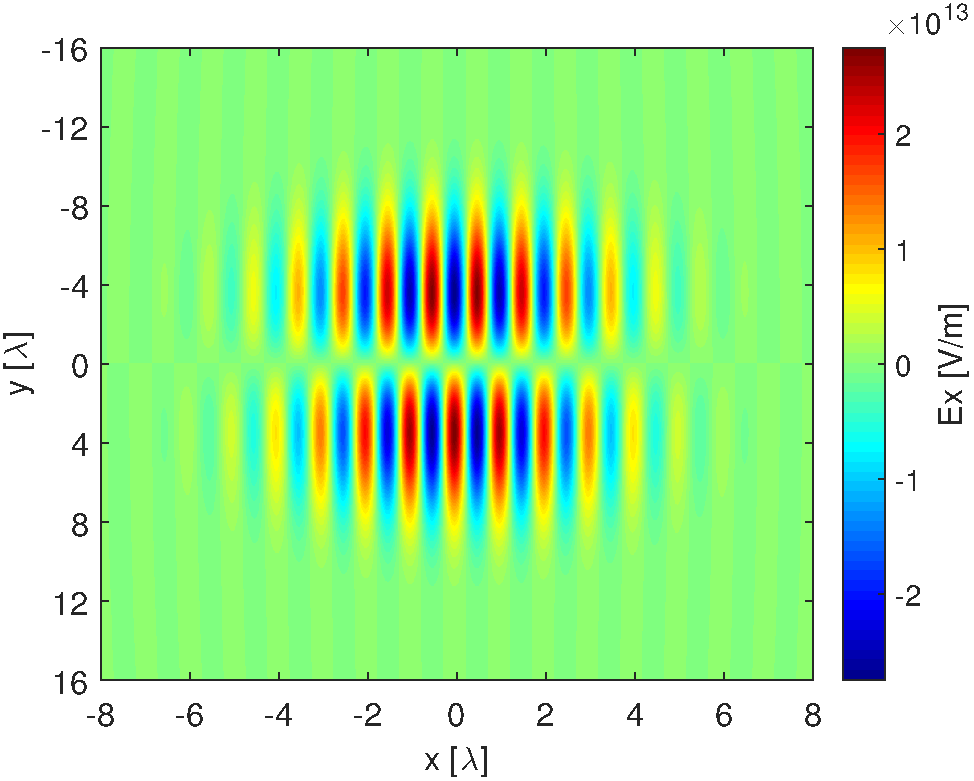
\includegraphics[width=0.44\linewidth]{./img/parax/Ex_focus_5mic.pdf}}}\\
	\sidesubfloat[]{{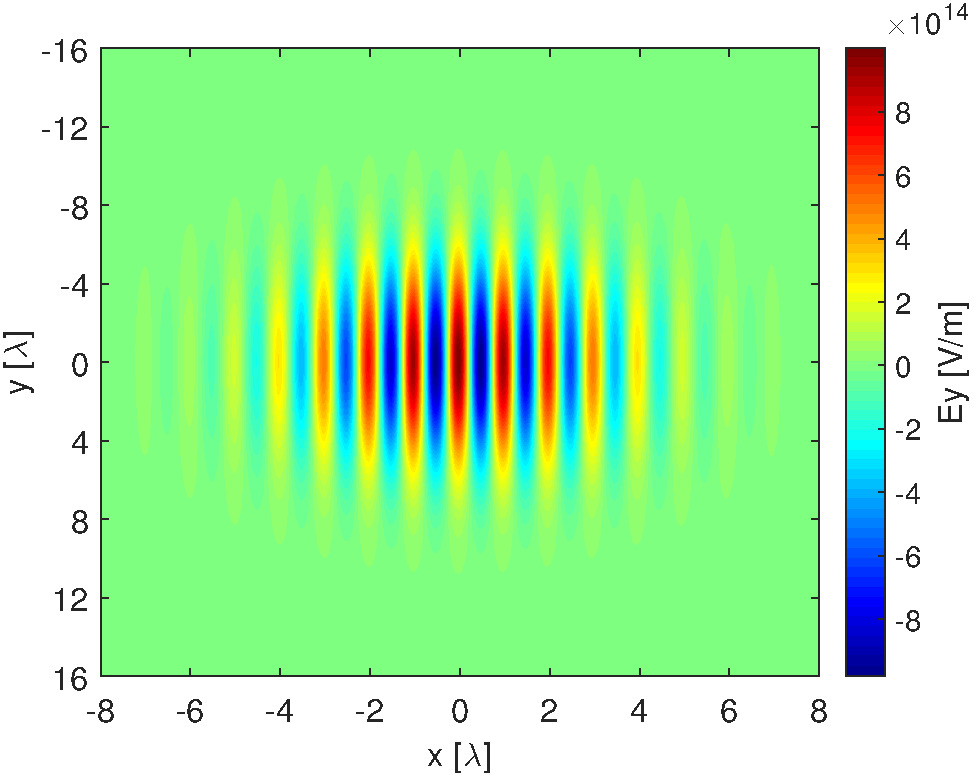
\includegraphics[width=0.44\linewidth]{./img/lbcs/Ey_focus_5mic.pdf}}}
	\hspace{2mm}
	\sidesubfloat[]{{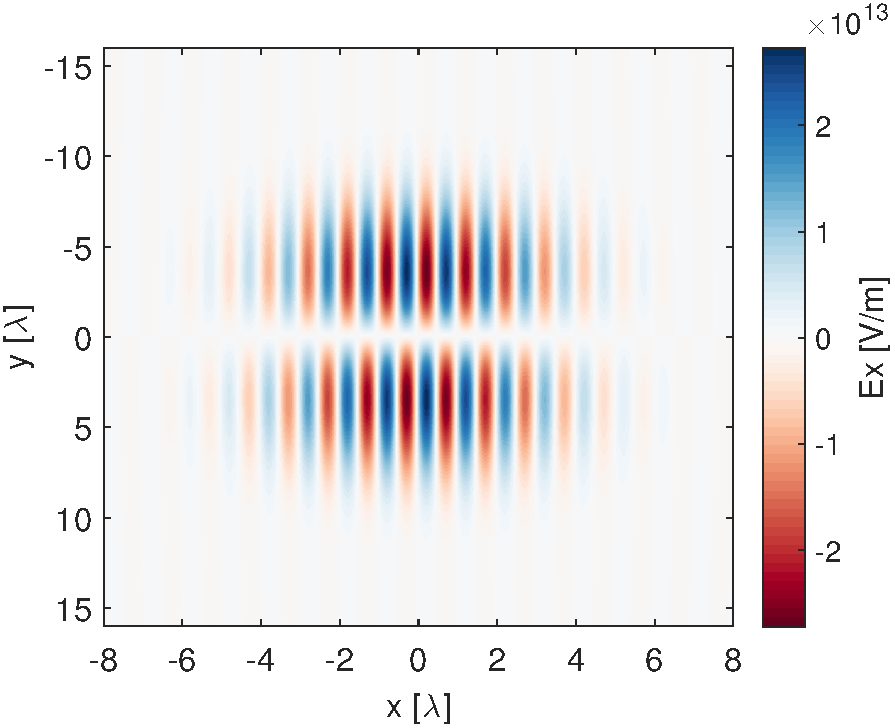
\includegraphics[width=0.43\linewidth]{./img/lbcs/Ex_focus_5mic.pdf}}}
	\caption{Transverse ($ E_{y} $) and longitudinal ($ E_{x} $) electric laser field components captured at the time step of their maximal intensity in the focal spot. The cases \textbf{(a)}, \textbf{(b)} correspond to the laser pulse propagating under the paraxial approximation, whilst \textbf{(c)}, \textbf{(d)} come from the simulation where the beam propagation has been resolved within the Maxwell consistent approach. The size of the focus has been chosen to be one order of the magnitude larger than the center laser wavelength. One can clearly see, that there is no significant difference between the shapes of the electric field components.}
	\label{fig:5}
\end{figure}

\floatsetup[figure]{style=plain, subcapbesideposition=top}
\begin{figure}[h!]
	\centering
	\sidesubfloat[]{{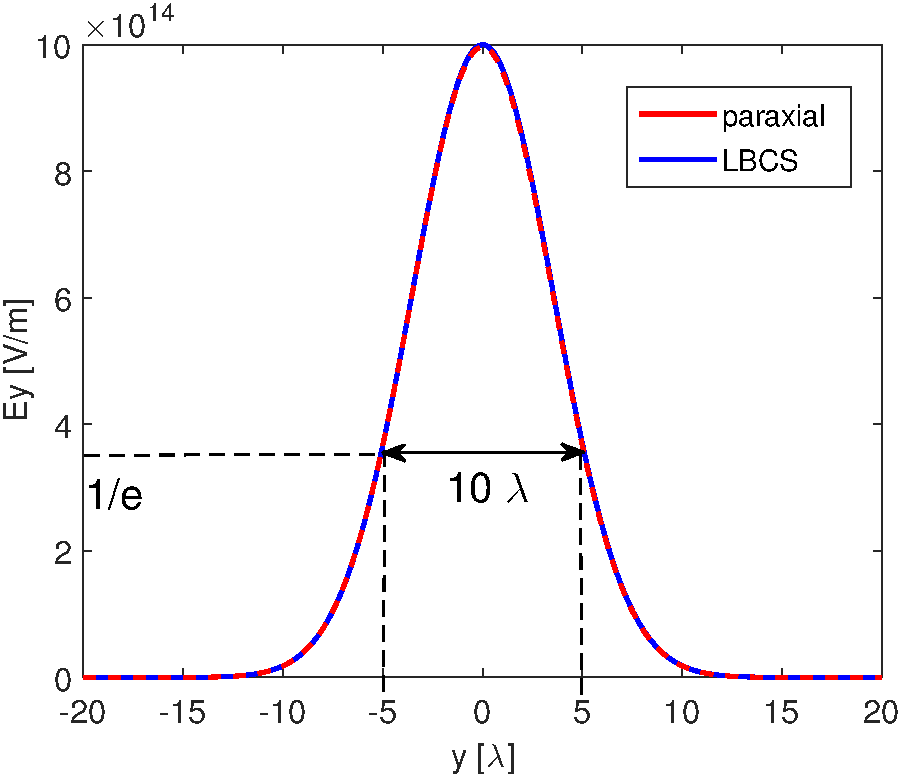
\includegraphics[width=0.4\linewidth]{./img/parax/Ey_focus_trans_comparison.pdf}}}
	\hspace{5mm}
	\sidesubfloat[]{{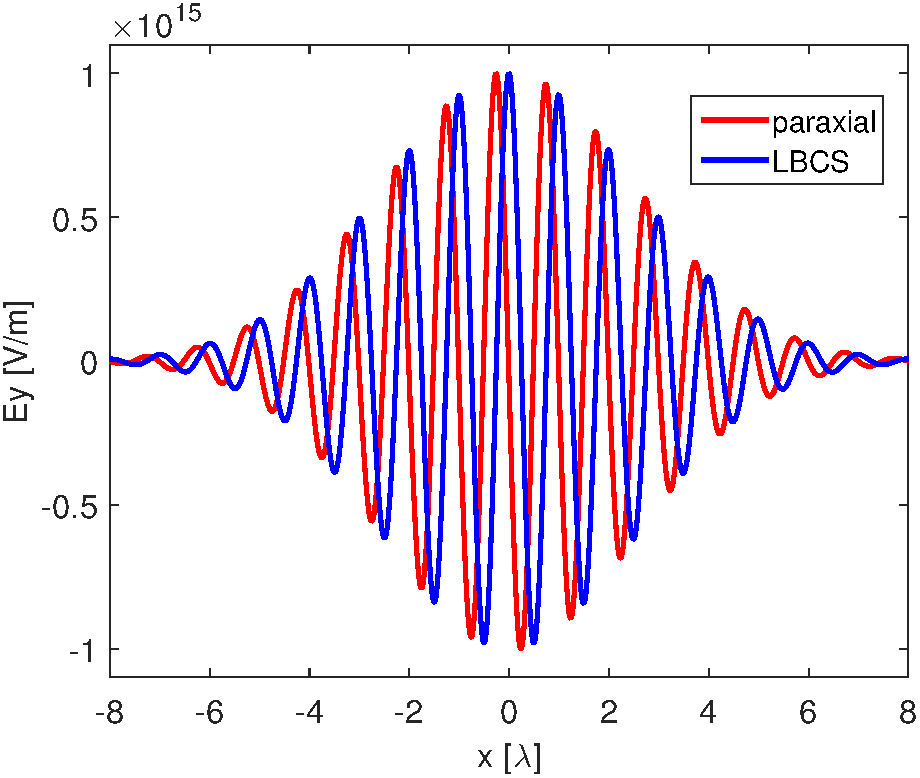
\includegraphics[width=0.4\linewidth]{./img/parax/Ey_focus_long_comparison.pdf}}}
	\caption{Transverse \textbf{(a)} and longitudinal \textbf{(b)} slices of the transverse electric laser field ($ E_{y} $) at the time step when it reaches maximal intensity in the focal spot. Red lines correspond to the laser pulse propagating under the paraxial approximation, whilst blue lines come from the simulation where the beam propagation has been resolved within the Maxwell consistent approach. The size of the focus has been chosen to be one order of magnitude larger than the center laser wavelength. In the case of paraxial approximation, the focus is slightly shifted closer to the left boundary \textbf{(b)}, otherwise the size of the focus as well as the amplitude is correct for both cases \textbf{(a)}.}
	\label{fig:6}
\end{figure}
